% CREATED BY DAVID FRISK, 2018
\chapter{Conclusion}
This chapter presents the conclusions drawn based on the analysis, empirical data and the theory. The important deductions are listed along with the future recommendations.
\begin{enumerate}
    \item Regarding the present twenty-three KPIs at PE-Sweden, the KPIs with high and medium impact must be continued to use with suggested improvements. Change KPIs need to be completely redefined. The KPIs under Trust and passion can be converted into action plans and be excluded from KPI list. The financial KPIs can be reduced in number and followed only by top management. Therefore, by adhering to all these conclusions the KPIs can be reduced in number and made to reflect business performance. Also the ones driving the wrong behaviours needed to be reconsidered by changing the way of measuring the KPIs.
    \item Using the AHP-SMART method the KPIs were analyzed to find the missing characteristics. Management knows what are the right characteristics for KPIs, but adapting them to their situation is the major challenge. Based on the comparison of literature and case the characteristics that needed focus were:
    \begin{itemize}
        \item Owned
        \item Easy to understand 
        \item Trigger changes
        \item Few in number
        \item Apart from these, the KPIs needed to be more SMARTer and more of leading KPIs.
    \end{itemize}
    
    \item Major learning from this thesis is that the supporting factors play a great role in effectiveness of the KPIs. The supporting factors which had a major impact in this case were Top Management interest, Strategic cascading, Visual communication and Performance measurement tools. Hence a KPI board model was created which could consolidate all the support factors which is presented in figure \ref{fig:final}. How the KPI board is envisioned is discussed below.\\
    \begin{figure}[H]
    \centering
    \captionsetup{justification=centering, margin=2cm}
    \vspace{1cm}
    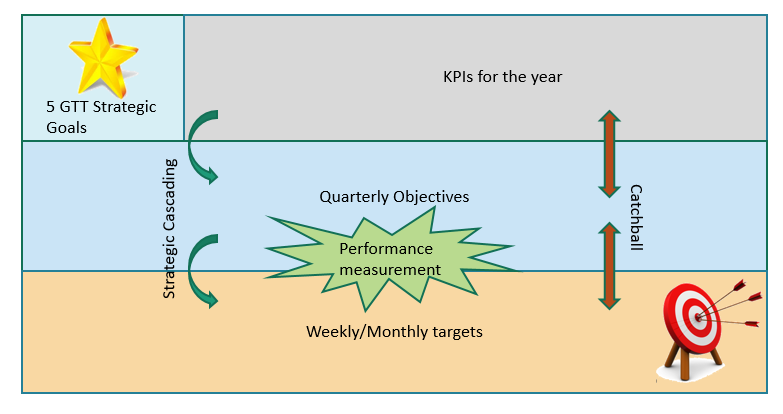
\includegraphics[width=13.5cm, height=7.5cm]{figure/auxiliary/final.PNG}
    \caption{KPI board}
    \label{fig:final}
\end{figure}
    %fig
    
    The 5 strategic priorities of GTT act as a north star to build the KPIs. Handful of KPIs are selected by top management for the year. It is important to ensure that these KPI align with the strategy and are applicable to most teams. These KPI targets are then broken down into quarterly objectives by catchball between the directors and group managers. This acts as a second step of strategic cascading. In the next step, teams together with their group manager can decide the objectives and key results for the quarter. These quarterly objectives are then broken down into weekly/monthly targets completing the strategic cascading. Also, this will automatically bring in awareness and participation of employees. Therefore, it satisfies all the important aspects such as Strategic cascading at all levels, Visual communication with the board, Top management interest by creating KPIs and following up on targets and better usage of performance measurement by OKR methodology.\\

Based on the conclusions of this thesis following future recommendations are given:
\begin{itemize}
    \item Pilot test of the KPI board could be done, and improved to make it more adaptable and effective before using it across PE-Sweden.
    \item The new KPIs for future could be developed keeping in mind the characteristics that need to be improved.
\end{itemize}

\end{enumerate}


